\documentclass[a4paper, 12pt]{article}
\usepackage[utf8]{inputenc}
\usepackage[T1]{fontenc}
\usepackage{times}
\usepackage[spanish]{babel}
% \usepackage{hyperref} % Paquete para hipervínculos
\usepackage[left=2.5cm, right=2.5cm, top=2.5cm, bottom=2.5cm]{geometry}
\linespread{1.5}
\usepackage{graphicx} % Required for inserting images
\usepackage{amsmath}
\usepackage{titlesec} % Paquete para el formato de los títulos
\usepackage{hyperref}

\setlength{\parindent}{0pt}

% Reducir el espacio entre los apartados del índice
\makeatletter
\renewcommand*\l@section{\@dottedtocline{1}{0em}{1.5em}}
\renewcommand*\l@subsection{\@dottedtocline{2}{1.5em}{2.5em}}
\renewcommand*\l@subsubsection{\@dottedtocline{3}{4.0em}{3.5em}}
\makeatother

\hypersetup{
	colorlinks=true,
	urlcolor=blue,
	linkcolor=black  % Cambia el color de los índices a azul oscuro
}

\begin{document}
%-------------------------------------------------------
% PORTADA
%-------------------------------------------------------
\begin{titlepage}
	\begin{center}
		
\includegraphics[scale=0.9]{images.png}
		\vspace{1.75cm}
		
		\large
		\textbf{ESCUELA TÉCNICA SUPERIOR DE INGENIERÍA INFORMÁTICA}
		\vspace{1cm}
		
		\large
		\textbf{GRADO EN INGENIERÍA INFORMÁTICA}
		
		
		
		\large
		\textbf{Curso Académico 2023/2024}
		
		\vspace{1cm}
		\large
		\textbf{Práctica 1}
		
		\vspace{2cm}
		
		\large
		\textbf{DETECCIÓN DE SEÑALES VIALES}
		
		\vspace{2cm}
		
		\large
		Cristian Fernando Calva Troya \\
		Luis Ovejero Martín \\
		Jaime Rueda Carpintero
		\vspace{1cm}
	\end{center}
\end{titlepage}

\newpage
\thispagestyle{empty} 
\mbox{} 

\newpage
%-------------------------------------------------------
% Tabla de figuras
%-------------------------------------------------------
\newpage
\listoffigures
\newpage

%-------------------------------------------------------
% Tabla de contenidos
%-------------------------------------------------------
{\small
	\tableofcontents 
}
\newpage

%-------------------------------------------------------
% 1. Introducción
%-------------------------------------------------------
\section{Introducción}
%-------------------------------------------------------
% 2. OBJETIVOS Y METODOLOGIAS
%-------------------------------------------------------
\section{Objetivos y metodología}

\subsection{Descripción del problema}

\subsection{Objetivos}
3 pag.
\subsection{Tecnologías}

%-------------------------------------------------------
% 3. DESCRIPCIÓN INFORMMATICA
%-------------------------------------------------------

\section{Creación de la aplicación}
\subsection{Ejercicio 1}

\subsection{Ejercicio 2}

\subsection{Ejercicio 3}
Una vez hemos conseguido entrenar un clasificador de caracteres y quedarnos con el que mejor resultados da, vamos a aplicar ese modelo a un caso más real que sería a la hora de detectar carteles de una autopista y clasificar los caracteres que se encuentran en el panel. La clase encargada de realizar toda esta parte de la lectura automática de los caracteres es \textit{main\_panels\_ocr.py}, donde llamando al método \textit{obtainRegionsDetected} podemos obtener los parámetros necesarios para la realización de este apartado. \\\\
Las imágenes con las que queremos realizar esta lectura son de unos carteles recortados de forma, orientación y relación de aspecto variable. Nuestro primer paso consiste en poder detectar los caracteres que luego vamos a clasificar. Para ello previamente vamos a normalizar el panel que le entre a este detector, donde primero cargaremos la imagen en escala de grises, aplicaremos un umbralizado adaptativo aplicando la Gaussiana y por último extraer los bordes de la imagen umbralizada. El proceso que se ha seguido se puede ver a partir de la \textbf{\hyperref[fig:normalizacion]{Fig. 1}}
\newpage
\begin{figure}[h]
	\centering
	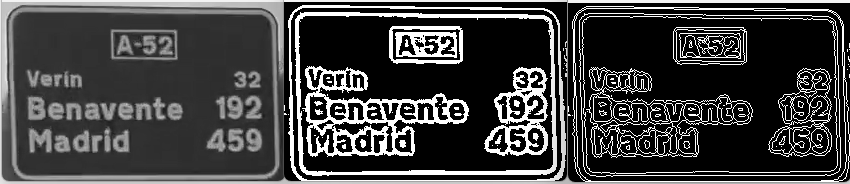
\includegraphics[width=0.8\linewidth]{img/imagenUmbral.png}
 	\caption{Proceso de normalización para la lectura de carteles}\vspace{0.5cm}
	\label{fig:normalizacion}
\end{figure}
Después de la umbralización, vamos a usar MSER para poder detectar las regiones más características de nuestra imagen, en este caso caracteres. La imagen se le pasará al método y antes de realizar el MSER realizaremos una dilatación para aumentar el grosor de los trazos de los caracteres. Los parámetros del MSER escogidos son los siguientes:
\begin{itemize}
    \item Delta = 5
    \item Variación máxima = 0.8
    \item Área mínima = 50
    \item Área máxima = 200
\end{itemize}
Lo más destacable de estos parámetros es la disminución de la ventana de las regiones detectadas debido a que nos encontramos con imágenes con bastante menos píxeles que las imágenes de la práctica anterior, donde nos encontrábamos con una imagen de toda la escena. El método deolverá una lista compuesta por las coordenadas de cada rectángulo detectado. En la \textbf{\hyperref[fig:normalizacion]{Fig. 2}} vemos cómo se comporta esta detección. 
\begin{figure}[h]
	\centering
	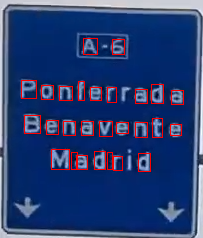
\includegraphics[width=0.2\linewidth]{img/deteccionMSER.png}
 	\caption{Carteles detectados con MSER}\vspace{0.5cm}
	\label{fig:normalizacion}
\end{figure}
\\Puede suceder que MSER detecte varias regiones que pertenecen a un mismo caracter. Esto se soluciona cuando se llama al método \textit{eliminateDuplicatedRectangles}, donde itera todos los rectágulos detectados y comprueba si dos de los rectángulos iterados se encuentran contenidos. Para saber eso se calcula un valor de IoU, donde a partir de un umbral podemos saber si dos rectángulos están superpuestos. Cuando nos encontremos en este caso, eliminaremos el rectángulo que abarque menos área y nos quedaremos con el más grande de los dos. Este bucle se recorrerá para todos los detectados.
\\\\
El paso siguiente consiste en poder agrupar los caracteres en palabras. Por ejemplo en el anterior cartel de la \textbf{\hyperref[fig:normalizacion]{Fig. 2}} a partir de los caracteres detectadas queremos formar el texto \textit{A6 Ponferrada Benavente Madrid}. La clase llama primero a la función \textit{computeCenters} que devolverá una lista con las coordenadas de los centros de los rectángulos. Esto se hace para poder ejecutar el algoritmo de RANSAC que se encargará de realizar esta agrupación. El método en cuestión es \textit{gropuCenters} y los parámetros serán los puntos y rectángulos a procesar y el número mínimo de muestras que compone una línea, donde en nuestro caso queremos formar palabras de más de 1 caracter, y un umbral de residuo que se utiliza para ajustar las líneas y diferenciar si una línea pertenece o no a un punto en función de su valor, que sería la distancia entre dos puntos. El algoritmo de RANSAC se aplicará a cada uno de los puntos. Para una mejor visión del algoritmo, nos centraremos en el ejemplo de la \textbf{\hyperref[fig:normalizacion]{Fig. 3}}.
\begin{figure}[h]
	\centering
	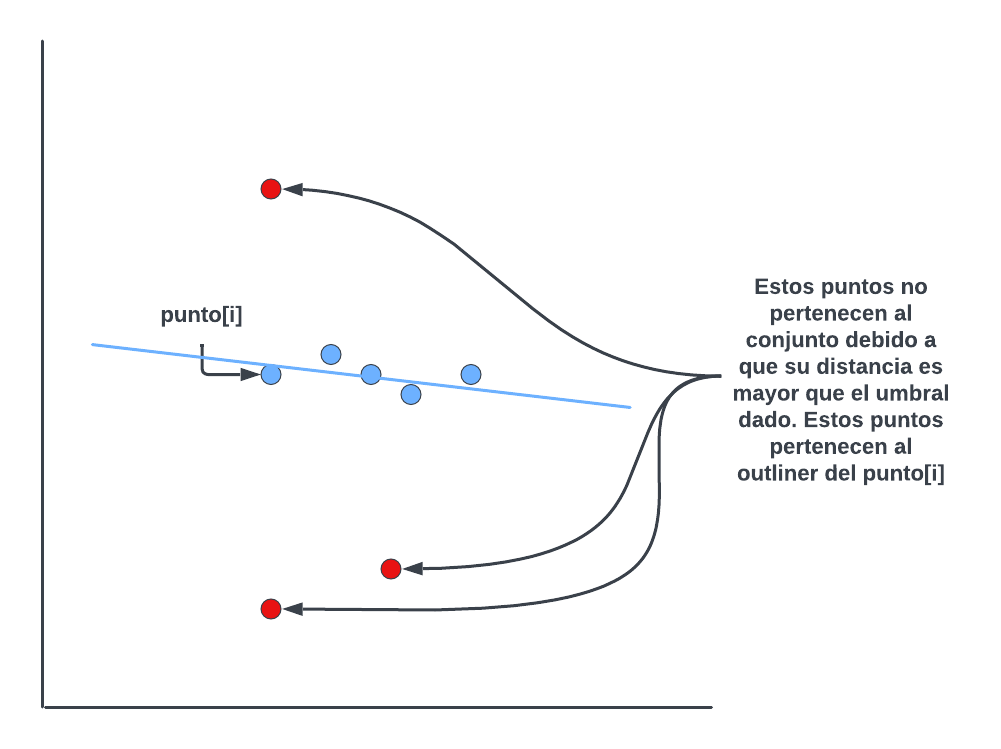
\includegraphics[width=0.6\linewidth]{img/RANSAC.png}
 	\caption{RANSAC aplicado a los puntos detectados}\
	\label{fig:normalizacion}
\end{figure}
\\ En la figura vemos que nos encontramos con el punto i de nuestro bucle. Sobre ese punto intentaremos obtener la línea de RANSAC a partir del umbral de residuo. Si un punto se encuentra a una mayor distancia que el umbral entonces el algoritmo no lo tendrá en cuenta a la hora de trazar la recta. Vemos que los puntos de arriba y abajo no deberían de pertenecer a la palabra ya que se encuentran más alejados que los que están en los puntos de en medio. La función de RANSAC tiene del método \textit{inlier\_mask} que permite calcular los puntos que pertenecen a la recta calculada. El método en cuestión devolverá una mascará que tendrá la misma longitud que la lista de los puntos y nos dirá  los puntos que se encuentran en el subconjunto. Esos puntos los almacenaremos en una lista de conjuntos y los marcaremos como explorados, para evitar que uno de los puntos obtenidos de la recta se itere otra vez. En el ejemplo la siguiente iteración será uno de los puntos de abajo o el de arriba ya que los puntos de en medio ya han sido explorados y se realizará el mismo proceso que lo anterior explicado. En este caso tendremos dos subconjuntos: los puntos de en medio y los puntos de abajo. El punto de arriba no ha sido agregado a ningún punto ya que los mínimos de puntos que hemos establecido para establecer la línea de RANSAC son dos. El proceso que se acaba de explicar, se puede ver a través de la siguiente figura \textbf{\hyperref[fig:puntosAgrupados]{Fig. 4}}.
\begin{figure}[h]
	\centering
	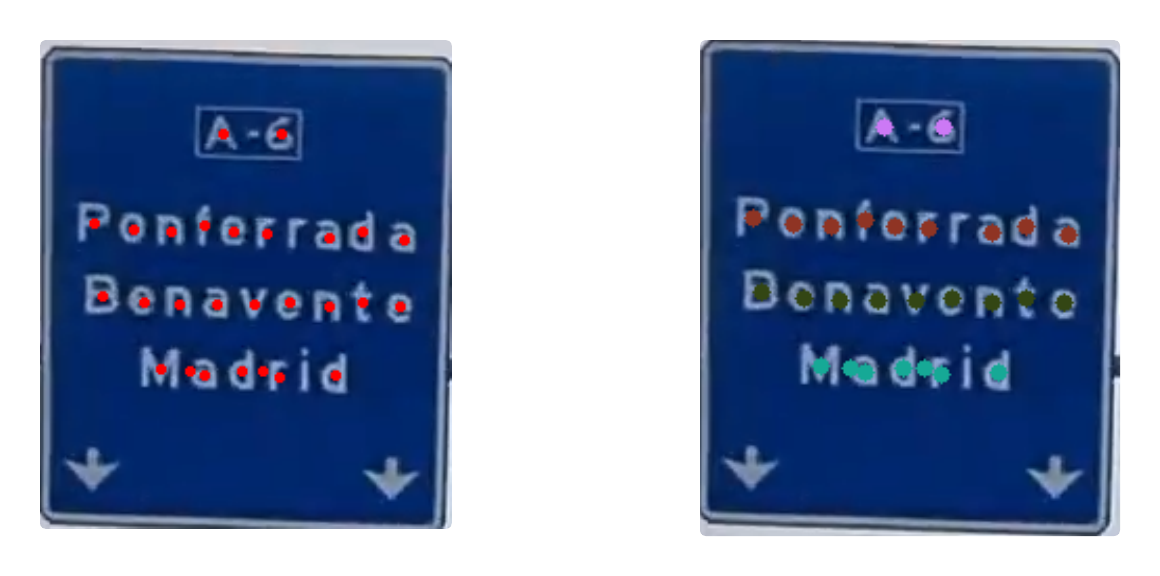
\includegraphics[width=0.6\linewidth]{img/puntosAgrupados.png}
 	\caption{Cálculo y agrupación de los centros de los rectángulos mediante RANSAC}\
	\label{fig:puntosAgrupados}
\end{figure}
\\El proceso de la detección de las palabras ya estaría completado, donde ya se han obtenido todas las líneas, rectangulos y centros detectados sobre la imagen, véase \textbf{\hyperref[fig:imagenDetectada]{Fig. 5}}. Nuestro último paso sería pasarle una lista de conjuntos de caracteres al clasificador para poder saber el tipo de caracter y así poder construir el texto del panel. Sin embargo, los paneles están desordenados, por lo que se construirá un texto erróneo ya que las palabras no están en orden. Para ello antes de realizar la clasificación se llama al método \textit{reorderRectangles}. El algoritmo es muy sencillo aunque es un tanto extenso. Las palabras deberían estar ordenadas en como leemos nostros el texto, de arriba a abajo, y los caracteres de izquierda a derecha. Primero reordenaremos las palabras para que estén de arriba a abajo. Para ello, nuestra variable \textit{clusterRectangles} es una lista 
\begin{figure}[h]
	\centering
	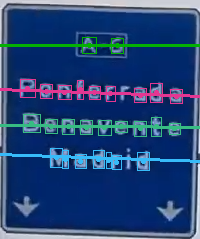
\includegraphics[width=0.2\linewidth]{img/detectionPanel.png}
 	\caption{Detección caracteres panel}\
	\label{fig:imagenDetectada}
\end{figure}
\\de listas, donde cada posición es la oración en sí. Iteraremos cada una de las oraciones y calcularemos su posición respecto al eje Y y reordenaremos esta lista de manera ascendente, donde las oraciones con menor Y irán primeras y las oraciones con mayor Y las últimas. Cabe destacar que en imágenes el punto (0,0) corresponde a la parte superior izquierda y es por esto por lo que se reordena en función del Y menor. Una vez hemos realizado el primer reordenamiento, podemos hacer el reordenamiento a nivel de caracter. Para ello en vez de usar los conjuntos de las listas, usaremos los conjuntos de los conjuntos de las listas, que representan a cada palabra de una oración. Sobre cada palabra aplicaremos un reordenamiento muy similar al anterior pero en este caso usando el eje X en lugar del Y. 
\end{document}
